\documentclass[11pt,a4paper]{article}
\usepackage[T1]{fontenc}
\usepackage[utf8]{inputenc}
\usepackage{lmodern}
\usepackage{textcomp}
\usepackage[left=1.8cm,right=1.8cm,top=3.0cm,bottom=2.2cm,headheight=36pt,headsep=12pt]{geometry}
\usepackage{multicol}
\usepackage{xcolor}
\usepackage{fancyhdr}\usepackage{tikz}
\usepackage{graphicx}
\usepackage{array}
\usepackage{amsmath,amssymb}
\usepackage{setspace}
\usepackage{longtable}
\graphicspath{{../}}
\definecolor{ygreen}{RGB}{46,139,87}\definecolor{dgreen}{RGB}{28,90,56}
\renewcommand{\normalsize}{\fontsize{10.9}{13.4}\selectfont}
\renewcommand{\familydefault}{\rmdefault}
\setlength{\parindent}{0pt}
\setlength{\columnsep}{0.8cm}
\setlength{\columnseprule}{0.4pt}
\setlength{\multicolsep}{3pt plus 1pt minus 1pt}
\renewcommand{\textsubscript}[1]{\ensuremath{_{\text{\fontsize{8}{8}\selectfont #1}}}}
\renewcommand{\textsuperscript}[1]{\ensuremath{^{\text{\fontsize{8}{8}\selectfont #1}}}}
\newcommand{\qn}[1]{\textbf{\fontsize{11.5}{13}\selectfont #1}}
\newcommand{\qsep}{\par\vspace{13pt}}
\newcommand{\fwrule}{\par\vspace{5pt}\noindent\rule{\linewidth}{1.4pt}\par\vspace{7pt}}
\newsavebox{\fitb}
\newcommand{\fitbox}[1]{\sbox{\fitb}{#1}\ifdim\wd\fitb>\linewidth\resizebox{\linewidth}{!}{\usebox{\fitb}}\else\usebox{\fitb}\fi}
\newcommand{\diqqat}[1]{\par\smallskip\noindent\textbf{Diqqat!} #1\par\medskip}
\newcommand{\javob}{\par\nopagebreak[4]\smallskip\noindent\textbf{Javob:} \rule[-2pt]{7.5cm}{0.4pt}\par\smallskip\noindent\textbf{Diqqat!} Javobingizni javoblar varaqasiga ko`chirib yozing.\par\medskip}
\pagestyle{fancy}
\fancyhf{}
\renewcommand{\headrulewidth}{1.6pt}\renewcommand{\headrule}{{\color{ygreen}\hrule height 1.6pt width\headwidth}}
\newcommand{\hdrlogo}{
\begin{tikzpicture}[baseline=0pt]\fill[ygreen,rounded corners=3pt] (0,0) rectangle (0.95,0.95);\node[white,font=\fontsize{24}{26}\bfseries\selectfont] at (0.475,0.47){K};\node[anchor=west,font=\fontsize{16}{18}\bfseries\selectfont,text=dgreen] at (1.15,0.66){KIMYO};\node[anchor=west,font=\footnotesize\scshape,text=gray] at (1.15,0.2){Milliy sertifikat\ \ 2026};\end{tikzpicture}}
\newcommand{\hdrpill}[1]{\begin{tikzpicture}[baseline=0pt]\node[fill=ygreen,text=white,rounded corners=8pt,inner xsep=10pt,inner ysep=5pt,font=\fontsize{13}{15}\bfseries\selectfont] at (0,0.475){#1};\end{tikzpicture}}
\fancyhead[L]{\hdrlogo}
\fancyhead[R]{\hdrpill{19-variant}}

\fancyfoot[C]{\thepage}
\fancypagestyle{first}{\fancyhf{}\renewcommand{\headrulewidth}{1.6pt}\renewcommand{\headrule}{{\color{ygreen}\hrule height 1.6pt width\headwidth}}\fancyhead[L]{\hdrlogo}\fancyhead[R]{\hdrpill{19-variant}}\fancyfoot[C]{\thepage}}
\begin{document}
\normalsize
\thispagestyle{first}
\noindent\textit{Davriy jadvaldan foydalanish mumkin.}
\par\smallskip
\begin{multicols}{2}
\noindent\qn{1.} Na\textsubscript{2}CO\textsubscript{3} eritmasida gidrolizlanish darajasini oshirish uchun qaysi usullar qo`llanadi? 1) NaOH eritmasi qo`shish; 2) qizdirish; 3) HCl qo`shish; 4) NH\textsubscript{4}Cl eritmasi qo`shish

\noindent A)~\textsl{1, 4} \hfill B)~\textsl{1, 2, 3} \hfill C)~\textsl{1, 3, 4} \hfill D)~\textsl{2, 3, 4}\par
\qsep
\noindent\qn{2.} pH = 11 bo`lgan eritmada gidroksid ionlari konsentratsiyasi 10\textsuperscript{$-$x} mol/l ga teng. x \textbf{ni aniqlang.}

\noindent A)~\textsl{11} \hfill B)~\textsl{4} \hfill C)~\textsl{10} \hfill D)~\textsl{3}\par
\qsep
\noindent\qn{3.} H\textsubscript{2}N--CH\textsubscript{2}--COOH molekulasidagi $\sigma$ va $\pi$ bog`lar \textbf{sonini aniqlang.}

\noindent A)~\textsl{9 va 1} \hfill B)~\textsl{8 va 1} \hfill C)~\textsl{9 va 2} \hfill D)~\textsl{10 va 1}\par
\qsep
\noindent\qn{4.} KClO\textsubscript{3} tarkibida Cl ning oksidlanish \textbf{darajasini aniqlang.}

\noindent A)~\textsl{+5} \hfill B)~\textsl{+3 va +5} \hfill C)~\textsl{$-$1} \hfill D)~\textsl{+4}\par
\qsep
\noindent\qn{5.} Kislotada Fe bo`lagi eritilganda ajralgan vodorod hajmining vaqtga bog`liqligi grafikda berilgan.
\begin{center}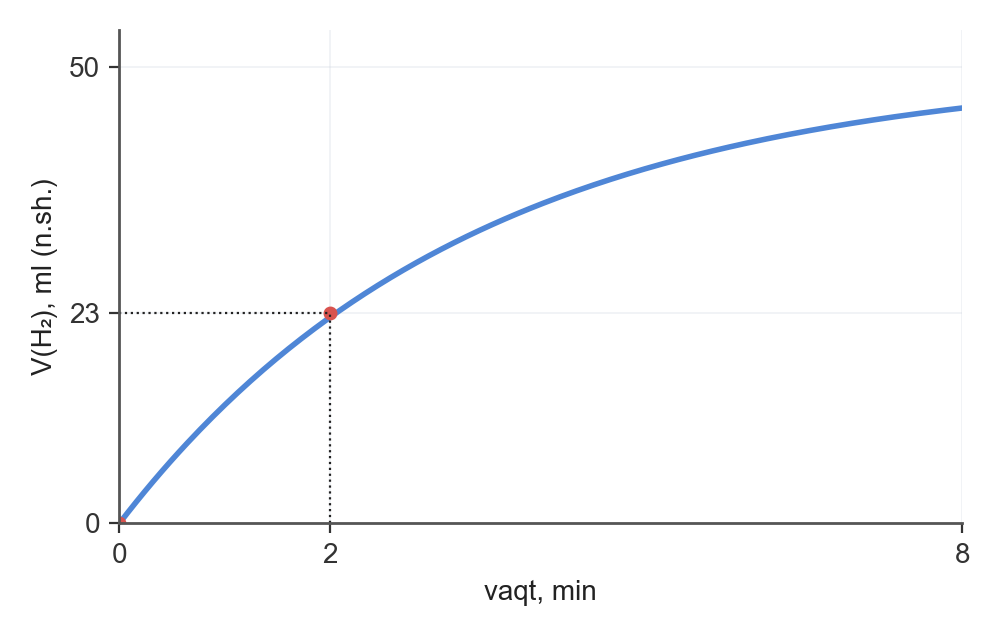
\includegraphics[width=0.86\linewidth]{rasmlar/gen/gv_v19_0.png}\end{center}
2-minutda ajralgan vodorodning \textbf{miqdorini (mmol) toping} (1 mmol gaz = 22,4 ml).

\noindent A)~\textsl{2,05} \hfill B)~\textsl{1,03} \hfill C)~\textsl{0,51} \hfill D)~\textsl{23}\par
\qsep
\noindent\qn{6.} 2 mol HCN va 1 mol C\textsubscript{4}H\textsubscript{6} (butadiyen-1,3) aralashmasidagi $\pi$-bog`lar umumiy \textbf{sonini (N\textsubscript{A} birligida) aniqlang.}

\noindent A)~\textsl{13} \hfill B)~\textsl{6} \hfill C)~\textsl{19} \hfill D)~\textsl{4}\par
\qsep
\noindent\qn{7.} 1 mol CH\textsubscript{4} tarkibidagi atomlar \textbf{sonini toping} (N\textsubscript{A} = 6,02$\cdot$10\textsuperscript{23}). Javobni 10\textsuperscript{23} birligida yozing.

\noindent A)~\textsl{6,02} \hfill B)~\textsl{1,505} \hfill C)~\textsl{3,01} \hfill D)~\textsl{0,602}\par
\qsep
\noindent\qn{8.} Faqat qaytaruvchi bo`la oladigan \textbf{ionlarni aniqlang}: 1) Fe\textsuperscript{3+}; 2) Mn\textsuperscript{7+} (MnO\textsubscript{4}\textsuperscript{$-$}); 3) Fe\textsuperscript{2+}; 4) Cl\textsuperscript{$-$}

\noindent A)~\textsl{1, 3} \hfill B)~\textsl{4} \hfill C)~\textsl{1, 4} \hfill D)~\textsl{1, 2}\par
\qsep
\noindent\qn{9.} N\textsubscript{2}O\textsubscript{4} $\rightleftarrows$ 2NO\textsubscript{2} reaksiyasi 2 l hajmli idishda o`tkazildi. Ma'lumotlar jadvalda berilgan:
\begin{center}
\renewcommand{\arraystretch}{1.15}
\fitbox{\begin{tabular}{|c|c|c|}\hline
\textbf{Modda} & \textbf{N\textsubscript{2}O\textsubscript{4}} & \textbf{NO\textsubscript{2}} \\ \hline
Boshlang`ich, mol & 4 & 0 \\ \hline
Muvozanatda, mol & --- & 3 \\ \hline
\end{tabular}}
\end{center}
N\textsubscript{2}O\textsubscript{4} ning necha foizi reaksiyaga \textbf{kirishganini aniqlang.}

\noindent A)~\textsl{18,8} \hfill B)~\textsl{56,2} \hfill C)~\textsl{37,5} \hfill D)~\textsl{62,5}\par
\qsep
\noindent\qn{10.} N\textsubscript{2} + O\textsubscript{2} $\rightleftarrows$ 2NO sistemasida boshlang`ich moddalarning har biridan 1 mol dan 2 l hajmli idishga solindi. Muvozanat qaror topganda reagentlarning har birining 3/4 qismi sarflangan bo`ldi. Muvozanat \textbf{konstantasini hisoblang.}

\noindent A)~\textsl{72} \hfill B)~\textsl{36} \hfill C)~\textsl{18} \hfill D)~\textsl{37}\par
\qsep
\noindent\qn{11.} H\textsubscript{2} va N\textsubscript{2} aralashmasi tarkibida aralashmadagi vodorod atomlari sonining azot atomlari soniga nisbati 3 : 2. Aralashmaning massasi 6,2 g. Aralashmadagi H\textsubscript{2} ning \textbf{massasini (g) toping.}

\noindent A)~\textsl{0,6} \hfill B)~\textsl{5,6} \hfill C)~\textsl{1,2} \hfill D)~\textsl{3,1}\par
\qsep
\noindent\qn{12.} Jadvalda NaOH ning ikki eritmasi haqida ma'lumot berilgan:
\begin{center}
\renewcommand{\arraystretch}{1.15}
\fitbox{\begin{tabular}{|c|c|c|}\hline
\textbf{Eritma} & \textbf{Massasi, g} & \textbf{Massa ulushi, \%} \\ \hline
1 & 200 & 5 \\ \hline
2 & 200 & 35 \\ \hline
\end{tabular}}
\end{center}
Eritmalar aralashtirilib, ustiga 100 g suv qo`shildi. Hosil bo`lgan eritmaning massa \textbf{ulushini (\%) aniqlang.}

\noindent A)~\textsl{20} \hfill B)~\textsl{40} \hfill C)~\textsl{16} \hfill D)~\textsl{14,4}\par
\qsep
\noindent\qn{13.} NaCl eritmasi inert elektrodlar bilan 10 A tok kuchi bilan 965 s elektroliz qilindi. Ajralgan gazlar aralashmasi yondirilib, hosil bo`lgan gaz 400 g suvda eritildi. Olingan kislota eritmasining massa \textbf{ulushini (\%) aniqlang.}

\noindent A)~\textsl{0,9} \hfill B)~\textsl{0,45} \hfill C)~\textsl{0,91} \hfill D)~\textsl{1,81}\par
\qsep
\noindent\qn{14.} Probirkalardagi eritmalar: Na\textsubscript{2}CO\textsubscript{3}, NaCl, Na\textsubscript{2}SO\textsubscript{4} ni alohida probirkalarda ajratish uchun qaysi reagent(lar) yetarli? 1) lakmus; 2) BaCl\textsubscript{2} va lakmus; 3) lakmus va fenolftalein; 4) BaCl\textsubscript{2}

\noindent A)~\textsl{3} \hfill B)~\textsl{1} \hfill C)~\textsl{2} \hfill D)~\textsl{1, 4}\par
\qsep
\noindent\qn{15.} Ishqoriy metallar haqida qaysi fikrlar to`g`ri? 1) Litiy eng yengil metall; 2) Natriy suv bilan reaksiyada H\textsubscript{2} va NaOH hosil qiladi; 3) Kaliy suvdan og`ir; 4) Ishqoriy metallar faqat oksidlovchi bo`ladi

\noindent A)~\textsl{1, 2} \hfill B)~\textsl{4} \hfill C)~\textsl{3, 4} \hfill D)~\textsl{2}\par
\qsep
\noindent\qn{16.} 0,2 mol fosfat kislota 0,5 mol NaOH bilan ta'sirlashtirildi (reagentlar to`liq sarflandi). Hosil bo`lgan tuzlar \textbf{massasini (g) hisoblang.}

\noindent A)~\textsl{28,4} \hfill B)~\textsl{32,8} \hfill C)~\textsl{61,2} \hfill D)~\textsl{30,6}\par
\qsep
\noindent\qn{17.} 1,2 mol xlorning yarmi sovuq, yarmi qaynoq KOH eritmasidan o`tkazildi (mo`l ishqor; sovuqda xlorid va gipoxlorit, qizdirilganda xlorid va xlorat hosil bo`ladi). Sarflangan KOH \textbf{massasini (g) aniqlang.}

\noindent A)~\textsl{67,2} \hfill B)~\textsl{268,8} \hfill C)~\textsl{201,6} \hfill D)~\textsl{134,4}\par
\qsep
\noindent\qn{18.} Zn va Ag aralashmasi (30,3 g) mo`l xlorid kislota bilan ta'sirlashganda 6,72 l (n.sh.) gaz ajraldi. Erimay qolgan qoldiq \textbf{massasini (g) aniqlang.}

\noindent A)~\textsl{10,8} \hfill B)~\textsl{19,5} \hfill C)~\textsl{15,2} \hfill D)~\textsl{21,6}\par
\qsep
\noindent\qn{19.} Reaksiya tenglamasi: Ca(HCO\textsubscript{3})\textsubscript{2} + Ca(OH)\textsubscript{2} $\to$ 2CaCO\textsubscript{3} + 2H\textsubscript{2}O. Reaksiyaga tarkibida 60\% aralashma bo`lgan 37 g namuna (asosiy modda Ca(OH)\textsubscript{2}) kirishdi. Ca(HCO\textsubscript{3})\textsubscript{2} \textbf{massasini (g) hisoblang.}

\noindent A)~\textsl{64,8} \hfill B)~\textsl{16,2} \hfill C)~\textsl{48,6} \hfill D)~\textsl{32,4}\par
\qsep
\noindent\qn{20.} Alken, alkadiyen va alkinlar haqida qaysi fikrlar to`g`ri? 1) Alkinlar uchun umumiy formula CnH\textsubscript{2}n+2; 2) Asetilenni Kucherov reaksiyasi bilan sirka aldegidiga aylantirish mumkin; 3) Propenga HBr birikishi Markovnikov qoidasiga bo`ysunadi; 4) Alkenlar KMnO\textsubscript{4} ning suvli eritmasi bilan glikol hosil qiladi

\noindent A)~\textsl{2, 3, 4} \hfill B)~\textsl{1, 2, 4} \hfill C)~\textsl{1, 3} \hfill D)~\textsl{2, 3}\par
\qsep
\noindent\qn{21.} Aldegid va ketonlar haqida qaysi fikrlar to`g`ri? 1) Sirka aldegid Kucherov reaksiyasi bilan olinadi; 2) Formalin --- formaldegidning 40\% li eritmasi; 3) Aldegidlar qaytarilganda ikkilamchi spirt hosil bo`ladi; 4) Aseton Cu(OH)\textsubscript{2} ni qaytaradi

\noindent A)~\textsl{2} \hfill B)~\textsl{1, 3, 4} \hfill C)~\textsl{1, 2} \hfill D)~\textsl{2, 4}\par
\qsep
\noindent\qn{22.} Uglevodlar haqida qaysi fikrlar to`g`ri? 1) Saxaroza Feling suyuqligini qaytaradi; 2) Glyukoza gidrolizlanadi; 3) Kraxmal va selluloza bir xil M ga ega; 4) Kraxmal yod bilan ko`k rang beradi

\noindent A)~\textsl{2} \hfill B)~\textsl{4} \hfill C)~\textsl{2, 4} \hfill D)~\textsl{1, 2}\par
\qsep
\noindent\qn{23.} 78 g benzol nitrolandi (unum 90\%), hosil bo`lgan nitrobenzol Zinin reaksiyasi bo`yicha qaytarildi (unum 80\%). Olingan anilin \textbf{massasini (g) hisoblang.}

\noindent A)~\textsl{133,9} \hfill B)~\textsl{33,5} \hfill C)~\textsl{93} \hfill D)~\textsl{67}\par
\qsep
\noindent\qn{24.} Propanol-1 va metanol aralashmasi (28 g) natriy bilan ta'sirlashganda 7,84 l (n.sh.) vodorod ajraldi. Aralashmadagi metanolning \textbf{massasini (g) aniqlang.}

\noindent A)~\textsl{6,4} \hfill B)~\textsl{30} \hfill C)~\textsl{16} \hfill D)~\textsl{32}\par
\qsep
\noindent\qn{25.} 90 g glukoza spirtli bijg`ishga uchradi (unum 80\%). Barcha reaksiyalar 2 atm bosimda olib borildi. Ajralgan gaz mo`l ohakli suvdan o`tkazilganda necha gramm cho`kma hosil bo`ladi?

\noindent A)~\textsl{100} \hfill B)~\textsl{40} \hfill C)~\textsl{80} \hfill D)~\textsl{160}\par
\qsep
\noindent\qn{26.} Rasmda benzol hosilasining tuzilish formulasi berilgan.
\begin{center}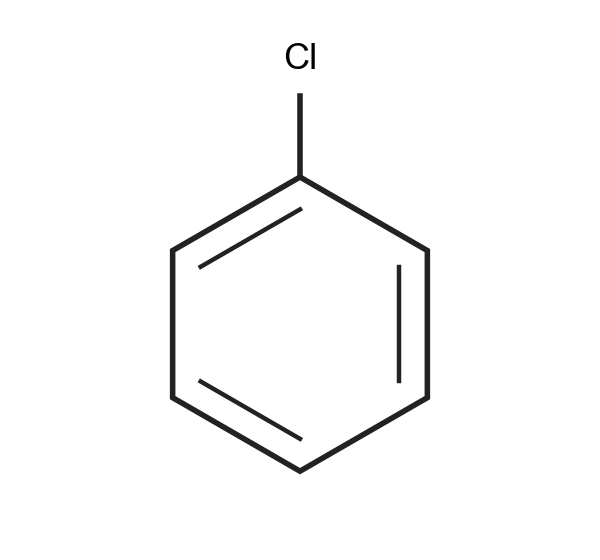
\includegraphics[width=0.86\linewidth]{rasmlar/gen/bs_976751.png}\end{center}
Birikmaning molekulyar \textbf{formulasini aniqlang.}

\noindent A)~\textsl{C\textsubscript{6}H\textsubscript{7}N} \hfill B)~\textsl{C\textsubscript{6}H\textsubscript{5}NO\textsubscript{2}} \hfill C)~\textsl{C\textsubscript{6}H\textsubscript{5}Cl} \hfill D)~\textsl{C\textsubscript{6}H\textsubscript{6}O}\par
\qsep
\noindent\qn{27.} To`yingan alifatik birlamchi amin yondirilganda hosil bo`lgan CO\textsubscript{2} hajmi azot hajmidan 8 marta ko`p bo`lsa, aminning molyar \textbf{massasini (g/mol) toping.}

\noindent A)~\textsl{73} \hfill B)~\textsl{87} \hfill C)~\textsl{59} \hfill D)~\textsl{90}\par
\qsep
\noindent\qn{28.} C\textsubscript{2}H\textsubscript{6} dan quyidagi sxema bo`yicha 45,06 g etilatsetat olindi: C\textsubscript{2}H\textsubscript{6} $\to$ C\textsubscript{2}H\textsubscript{4} $\to$ C\textsubscript{2}H\textsubscript{5}OH $\to$ CH\textsubscript{3}COOC\textsubscript{2}H\textsubscript{5}. Bosqichlarning unumi ketma-ket 40\%, 80\%, 40\% ni tashkil qiladi. Barcha reaksiyalar 2 atm bosimda olib borildi. Sarflangan C\textsubscript{2}H\textsubscript{6} hajmi (l, n.sh.) \textbf{ni aniqlang.}

\noindent A)~\textsl{179,2} \hfill B)~\textsl{89,6} \hfill C)~\textsl{44,8} \hfill D)~\textsl{35,84}\par
\qsep
\noindent\qn{29.} C\textsubscript{3}H\textsubscript{8} dan quyidagi sxema bo`yicha 157,76 g aseton olindi: C\textsubscript{3}H\textsubscript{8} $\to$ CH\textsubscript{3}--CH=CH\textsubscript{2} $\to$ CH\textsubscript{3}--CH(OH)--CH\textsubscript{3} $\to$ CH\textsubscript{3}--CO--CH\textsubscript{3}. Bosqichlarning unumi ketma-ket 85\%, 80\%, 40\% ni tashkil qiladi. Sarflangan C\textsubscript{3}H\textsubscript{8} hajmi (l, n.sh.) \textbf{ni aniqlang.}

\noindent A)~\textsl{448} \hfill B)~\textsl{224} \hfill C)~\textsl{112} \hfill D)~\textsl{190,4}\par
\qsep
\noindent\qn{30.} Rasmdagi tajribada hosil bo`lgan gaz bromli suvdan o`tkazilganda nima kuzatiladi?
\begin{center}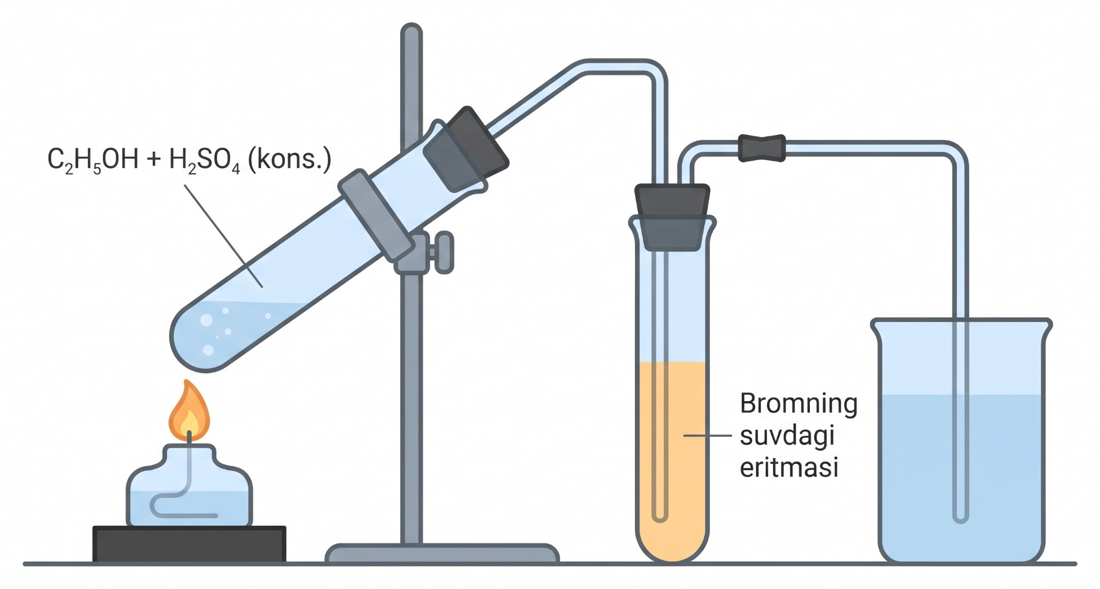
\includegraphics[width=0.86\linewidth]{rasmlar/darslik/d_etilen.png}\end{center}
\noindent A)~\textsl{bromli suv ko`k rangga kiradi}\par
\noindent B)~\textsl{cho`kma hosil bo`ladi}\par
\noindent C)~\textsl{o`zgarish bo`lmaydi}\par
\noindent D)~\textsl{bromli suv rangsizlanadi}\par
\qsep
\noindent\qn{31.} Quyidagi jarayonlar qanday kuzatuvlar bilan boradi? To`g`ri ta'riflangan \textbf{jarayonlarni belgilang.} 1) ZnSO\textsubscript{4} eritmasiga avval oz, so`ng mo`l NaOH eritmasi qo`shilganda: oq cho`kma tushadi, keyin cho`kma erib ketadi; 2) NaOH eritmasiga CuSO\textsubscript{4} eritmasi tomchilab qo`shilganda (ishqor mo`l): ko`k cho`kma tushadi, keyin ko`k cho`kma hosil bo`ladi va erimaydi; 3) CuSO\textsubscript{4} eritmasiga avval NaOH, so`ng mo`l ammiak eritmasi qo`shilganda: ko`k cho`kma tushadi, keyin cho`kma erib, to`q ko`k eritma hosil bo`ladi; 4) AgNO\textsubscript{3} eritmasiga avval NaCl, so`ng mo`l ammiak eritmasi qo`shilganda: oq tvorogsimon cho`kma tushadi, keyin cho`kma sariq tusga kiradi

\noindent A)~\textsl{1, 3, 4} \hfill B)~\textsl{3, 4} \hfill C)~\textsl{1, 2, 4} \hfill D)~\textsl{1, 2, 3}\par
\qsep
\noindent\qn{32.} Lakmus indikatori kislotali muhitda qanday rang beradi?
\noindent A)~\textsl{binafsha}\par
\noindent B)~\textsl{qizil}\par
\noindent C)~\textsl{rangsiz}\par
\noindent D)~\textsl{malina rangga kiradi (pushti)   ---}\par
\qsep
\end{multicols}
\medskip
\noindent\setlength{\fboxsep}{0pt}\fbox{\begin{tabular}{p{0.74\linewidth}|p{0.2\linewidth}}
\parbox[t]{0.72\linewidth}{\vspace{3pt}\textbf{Topshiriqlar (33--35) va javob variant (A--F)larini o`zaro to`g`ri moslashtiring.} 0,4 mol/l li NaCl eritmasining 1000 ml i inert elektrodlar yordamida 5 A tok kuchi bilan 1930 s elektroliz qilindi (eritma hajmi o`zgarmadi deb hisoblang). Ajralgan gazlar aralashmasi yondirilib, hosil bo`lgan gaz 100 g suvda eritildi.
\vspace{3pt}} & \parbox[t]{0.19\linewidth}{\vspace{3pt}A~\textsl{3,52}\\[3pt]
B~\textsl{13}\\[3pt]
C~\textsl{26}\\[3pt]
D~\textsl{0,3}\\[3pt]
E~\textsl{7,04}\\[3pt]
F~\textsl{2,82}}\\ \hline
\parbox[t]{0.72\linewidth}{\vspace{2pt}\textbf{33. Elektrolizdan keyin eritmaning pH ini hisoblang.}\vspace{2pt}} & \\ \hline
\parbox[t]{0.72\linewidth}{\vspace{2pt}\textbf{34. Elektrolizdan keyin eritmada NaCl ning molyar konsentratsiyasini (mol/l) toping.}\vspace{2pt}} & \\ \hline
\parbox[t]{0.72\linewidth}{\vspace{2pt}\textbf{35. Olingan xlorid kislota eritmasining massa ulushini (\%) aniqlang.}\vspace{2pt}} & 
\end{tabular}}
\par\bigskip
\noindent\qn{36.} 30\% li va 10\% li tuz eritmalari massalar nisbati 3 : 2 bo`lgan holda aralashtirildi. Tajriba hajmi 1000 ml bo`lgan kolbada o`tkazildi. Hosil bo`lgan eritmaning massa \textbf{ulushini (\%) hisoblang.}
\javob\qsep
\noindent\qn{37.} CO + H\textsubscript{2}O $\rightleftarrows$ CO\textsubscript{2} + H\textsubscript{2} sistemasida boshlang`ich moddalarning har biridan 2 mol dan 1 l hajmli idishga solindi. Muvozanat qaror topganda reagentlarning har birining 3/4 qismi sarflangan bo`ldi. Tajriba laboratoriyada, kvars idishda o`tkazildi. Muvozanat \textbf{konstantasini hisoblang.}
\javob\qsep
\noindent\qn{38.} Oksidlanish darajasi +3 bo`lgan noma'lum \textit{X} metallning xloridi 8,12 g massada mo`l AgNO\textsubscript{3} eritmasi bilan ta'sirlashganda 21,53 g cho`kma hosil bo`ldi. Reagent (AgNO\textsubscript{3}) eritmasining massa ulushi 10\% va zichligi 1,4 g/ml; u mo`l miqdorda olingan. \textit{X} metallning nisbiy atom \textbf{massasini toping.}
\javob\qsep
\noindent\qn{39.} 22,4 l (n.sh.) atsetilen Kucherov reaksiyasi bo`yicha gidratlandi (unum 1/2); hosil bo`lgan aldegidning 3/5 qismi ammiakli kumush oksid eritmasi bilan qizdirildi. Qizdirish 20 daqiqa davom etdi. Ajralgan kumush \textbf{massasini (g) hisoblang.}
\javob\qsep
\noindent\qn{40.} Bir atomli to`yingan noma'lum spirtning 18,4 g miqdori natriy bilan ta'sirlashganda 4,48 l (n.sh.) vodorod ajraldi. Shu spirtning 3/4 qismi mis(II) oksid bilan oksidlandi, hosil bo`lgan modda mo`l ammiakli kumush oksid eritmasi bilan qizdirildi. Qizdirish 30 daqiqa davom etdi. Ajralgan kumush \textbf{massasini (g) toping.}
\javob\qsep
\par\bigskip\begin{center}\textbf{\fontsize{13}{15}\selectfont YOZMA ISH}\end{center}
\noindent\qn{41.} \textbf{Topshiriqni bajarish jarayonida barcha reaksiya tenglamalarini yozing. Miqdoriy va arifmetik hisoblashlarni (unga asos bo`lgan usul yoki formulani ko`rsatgan holda) uzviy ketma-ketlikda bajaring.}\par\smallskip
Tarkibi FeSO\textsubscript{4}$\cdot$nH2O bo`lgan kristallogidratning 12,1 g namunasi suvda eritildi va unga sulfat kislota hamda 25 g 3,4\% li vodorod peroksid eritmasi qo`shildi (H\textsubscript{2}O\textsubscript{2} va H\textsubscript{2}SO\textsubscript{4} qoldiqsiz sarflandi, Fe\textsuperscript{2+} to`liq oksidlandi). Hosil bo`lgan eritmaga mo`l NaOH eritmasi qo`shilib, cho`kma ajratildi va doimiy massagacha kuydirildi. Kuydirish vaqtida ajralgan suv bug`i 127 \textdegree{}C va 83,14 kPa da o`lchandi (R = 8,314 J/(mol$\cdot$K)).\par
\noindent 1)\ Oksidlash, cho`ktirish va kuydirish reaksiyalarining tenglamalarini yozing va tenglashtiring.\par
\noindent 2)\ Kristallogidratdagi n ni aniqlang (tarkibini yozing).\par
\noindent 3)\ Kuydirishdan hosil bo`lgan qattiq moddaning massasini (g) toping.\par
\noindent 4)\ Fe\textsuperscript{3+} ni to`liq cho`ktirish uchun sarflangan NaOH miqdorini (mol) hisoblang.\par
\noindent 5)\ Kuydirishda ajralgan suv bug`ining hajmini (l) aniqlang.\par
\diqqat{Mazkur topshiriq kengaytirilgan javobni talab etib, uning yechilish usuli va shu usul asosidagi barcha hisoblash amallari javoblar varaqasida aks etishi lozim.}\qsep
\noindent\qn{42.} Organik moddalarning xossalarini bilgan holda reaksiya tenglamalarini tugallang va tenglashtiring. 3- va 5-reaksiyalarda hosil bo`lgan asosiy organik mahsulotlarni sistematik nomenklatura bo`yicha nomlang. Hosil bo`lgan organik moddalarning tuzilish formulalarini yozing.\par
\noindent 1)\ CH\textsubscript{3}--COOH + Cl\textsubscript{2} (P, t) $\to$\par
\noindent 2)\ C\textsubscript{6}H\textsubscript{5}--OH + Br\textsubscript{2} (suvli eritma) $\to$\par
\noindent 3)\ H\textsubscript{2}N--CH\textsubscript{2}--COOH + HCl $\to$\par
\noindent 4)\ CH\textsubscript{3}--CH\textsubscript{2}--OH (H\textsubscript{2}SO\textsubscript{4} kons., 170 \textdegree{}C) $\to$\par
\noindent 5)\ H\textsubscript{2}N--CH\textsubscript{2}--COOH + NaOH $\to$\par
\noindent 6)\ CH\textsubscript{3}--CH(OH)--CH\textsubscript{3} + CuO (t) $\to$\par
\noindent 7)\ CH$\equiv$CH + H\textsubscript{2}O (Hg\textsuperscript{2+}, H\textsuperscript{+}) $\to$\par
\diqqat{Mazkur topshiriq kengaytirilgan javobni talab etib, uning yechilish usuli va shu usul asosidagi barcha hisoblash amallari javoblar varaqasida aks etishi lozim.}\qsep
\noindent\qn{43.} \textbf{Topshiriqni bajarish jarayonida barcha reaksiya tenglamalarini yozing. Miqdoriy va arifmetik hisoblashlarni (unga asos bo`lgan usul yoki formulani ko`rsatgan holda) uzviy ketma-ketlikda bajaring.}\par\smallskip
CaCO\textsubscript{3} va MgCO\textsubscript{3} dan iborat aralashmada ularning massalari nisbati 25 : 7. Aralashma doimiy massagacha qizdirilganda massasi 17,6 g ga kamaydi. Ajralgan gaz 0,5 mol NaOH saqlagan eritmaga yuttirildi (gaz to`liq yutildi), hosil bo`lgan eritmaga mo`l BaCl\textsubscript{2} eritmasi qo`shildi. Qizdirishdan qolgan qattiq qoldiq esa 10\% li xlorid kislotaning stexiometrik miqdorida eritildi. Reagent (BaCl\textsubscript{2}) eritmasining massa ulushi 10\% va zichligi 1,3 g/ml; u mo`l miqdorda olingan. Qoldiqning HCl dagi eritmasiga mo`l Na\textsubscript{2}CO\textsubscript{3} eritmasi qo`shilib, hosil bo`lgan cho`kma ajratildi va doimiy massagacha qizdirildi; ajralgan gaz mo`l ohakli suvga yuborildi.\par
\noindent 1)\ Barcha reaksiyalarning tenglamalarini yozing va tenglashtiring. Dastlabki aralashmadagi karbonatlarning massalarini (g) aniqlang.\par
\noindent 2)\ Ajralgan gazning hajmini (l, n.sh.) hisoblang va hosil bo`lgan tuzlar tarkibini (o`rta/nordon) aniqlang.\par
\noindent 3)\ Gaz yutilgandan keyingi eritmadagi tuzlarning massalarini (g) toping. Na\textsubscript{2}CO\textsubscript{3} qo`shilganda hosil bo`lgan cho`kmalarning umumiy massasini (g) hisoblang.\par
\noindent 4)\ BaCl\textsubscript{2} qo`shilganda hosil bo`lgan cho`kma massasini (g) hisoblang. Cho`kma qizdirilganda massa necha gramga kamayadi?\par
\noindent 5)\ Qoldiq erigan eritmaning massasini (g) va undagi tuzlarning massa ulushlarini (\%) toping. Ohakli suvga yuborilganda hosil bo`lgan cho`kma massasini (g) toping.\par
\diqqat{Mazkur topshiriq kengaytirilgan javobni talab etib, uning yechilish usuli va shu usul asosidagi barcha hisoblash amallari javoblar varaqasida aks etishi lozim.}\qsep
\newpage
\noindent\textbf{\fontsize{13}{15}\selectfont 19-variant}\hfill \textbf{Javoblar kaliti}\par\smallskip\hrule\smallskip
\textit{Faqat o`qituvchi uchun.}\par\medskip
\noindent\textbf{1--32-savollar}\par\smallskip
\noindent\begin{tabular}{|c|c|c|c|c|c|c|c|c|c|c|c|c|c|c|c|}\hline
\textbf{1} & \textbf{2} & \textbf{3} & \textbf{4} & \textbf{5} & \textbf{6} & \textbf{7} & \textbf{8} & \textbf{9} & \textbf{10} & \textbf{11} & \textbf{12} & \textbf{13} & \textbf{14} & \textbf{15} & \textbf{16}\\\hline
\textsl{D} & \textsl{D} & \textsl{A} & \textsl{A} & \textsl{B} & \textsl{B} & \textsl{C} & \textsl{B} & \textsl{C} & \textsl{B} & \textsl{A} & \textsl{C} & \textsl{A} & \textsl{C} & \textsl{A} & \textsl{D}\\\hline
\textbf{17} & \textbf{18} & \textbf{19} & \textbf{20} & \textbf{21} & \textbf{22} & \textbf{23} & \textbf{24} & \textbf{25} & \textbf{26} & \textbf{27} & \textbf{28} & \textbf{29} & \textbf{30} & \textbf{31} & \textbf{32}\\\hline
\textsl{D} & \textsl{A} & \textsl{D} & \textsl{A} & \textsl{C} & \textsl{B} & \textsl{D} & \textsl{C} & \textsl{C} & \textsl{C} & \textsl{A} & \textsl{B} & \textsl{B} & \textsl{D} & \textsl{D} & \textsl{B}\\\hline
\end{tabular}\par\medskip
\noindent\textbf{33--35-savollar}\par\smallskip
\noindent\begin{tabular}{|c|c|c|}\hline \textbf{No} & \textbf{Javob} & \textbf{Qiymat}\\\hline
33 & \textsl{B} & 13\\\hline
34 & \textsl{D} & 0,3\\\hline
35 & \textsl{A} & 3,52\\\hline
\end{tabular}\par\medskip
\noindent\textbf{36--40-savollar}\par\smallskip
\noindent\begin{tabular}{|c|c|}\hline \textbf{No} & \textbf{To`g`ri javob}\\\hline
36 & 22\\\hline
37 & 9\\\hline
38 & 56\\\hline
39 & 64,8\\\hline
40 & 64,8\\\hline
\end{tabular}\par\medskip
\noindent\textbf{41--43-topshiriqlar: javoblar}\par\smallskip
\noindent\textbf{41-topshiriq.}\par
\noindent 1) 2FeSO\textsubscript{4} + H\textsubscript{2}O\textsubscript{2} + H\textsubscript{2}SO\textsubscript{4} $\to$ Fe\textsubscript{2}(SO\textsubscript{4})\textsubscript{3} + 2H\textsubscript{2}O; Fe\textsubscript{2}(SO\textsubscript{4})\textsubscript{3} + 6NaOH $\to$ 2Fe(OH)\textsubscript{3}$\downarrow$ + 3Na\textsubscript{2}SO\textsubscript{4}; 2Fe(OH)\textsubscript{3} $\to$ Fe\textsubscript{2}O\textsubscript{3} + 3H\textsubscript{2}O (t)\par
\noindent 2) FeSO\textsubscript{4}$\cdot$5H\textsubscript{2}O\par
\noindent 3) 4 g\par
\noindent 4) 0,15 mol\par
\noindent 5) 3 l\par
\noindent\textbf{42-topshiriq.}\par
\noindent 1) CH\textsubscript{3}--COOH + Cl\textsubscript{2} $\to$ CH\textsubscript{2}Cl--COOH + HCl\par
\noindent 2) C\textsubscript{6}H\textsubscript{5}--OH + 3Br\textsubscript{2} $\to$ C\textsubscript{6}H\textsubscript{2}Br\textsubscript{3}--OH$\downarrow$ + 3HBr\par
\noindent 3) H\textsubscript{2}N--CH\textsubscript{2}--COOH + HCl $\to$ [H\textsubscript{3}N--CH\textsubscript{2}--COOH]Cl --- nomi: \textbf{glitsin gidroxloridi}\par
\noindent 4) CH\textsubscript{3}--CH\textsubscript{2}--OH $\to$ CH\textsubscript{2}=CH\textsubscript{2} + H\textsubscript{2}O\par
\noindent 5) H\textsubscript{2}N--CH\textsubscript{2}--COOH + NaOH $\to$ H\textsubscript{2}N--CH\textsubscript{2}--COONa + H\textsubscript{2}O --- nomi: \textbf{natriy aminoetanoat (glitsinat)}\par
\noindent 6) CH\textsubscript{3}--CH(OH)--CH\textsubscript{3} + CuO $\to$ CH\textsubscript{3}--CO--CH\textsubscript{3} + Cu + H\textsubscript{2}O\par
\noindent 7) CH$\equiv$CH + H\textsubscript{2}O $\to$ CH\textsubscript{3}--CHO\par
\noindent\textbf{43-topshiriq.}\par
\noindent 1) 30 g; 8,4 g\par
\noindent 2) 8,96 l\par
\noindent 3) 10,6 g; 25,2 g; 38,4 g\par
\noindent 4) 19,7 g; 17,6 g\par
\noindent 5) 312,8 g; 10,65\%; 3,04\%; 40 g\par
\par\bigskip\noindent\textbf{Mavzular taqsimoti}\par\smallskip
{\small\noindent\begin{longtable}{|c|p{7.2cm}|p{5.4cm}|c|}\hline \textbf{No} & \textbf{Mavzu} & \textbf{Tekshiriladigan ko`nikma} & \textbf{Ball}\\\hline
1 & 9-sinf; 11-sinf (tuzlar gidrolizi; Le-Shatelye) & Bilim va tushunish & 1\\\hline
2 & Tirkashev IV bob (suvning ion ko`paytmasi) & Hisoblash va masala yechish & 1\\\hline
3 & 10-sinf \S{}17 (gibridlanish); Abdusamatov & Bilim va tushunish & 1\\\hline
4 & 8-sinf; Tirkashev \textit{V} bob (oksidlanish darajasi) & Bilim va tushunish & 1\\\hline
5 & Tirkashev VI bob (reaksiya tezligi, grafik) & Grafik tahlili & 1\\\hline
6 & 8-10-sinf ($\sigma$- va $\pi$-bog`lar) & Hisoblash va masala yechish & 1\\\hline
7 & 7-sinf (Avogadro) & Hisoblash va masala yechish & 1\\\hline
8 & Tirkashev \textit{V} bob; 11-sinf 7-bob & Bilim va tushunish & 1\\\hline
9 & Tirkashev VI bob (muvozanat, jadval) & Jadval tahlili & 1\\\hline
10 & 9-11-sinf (kimyoviy muvozanat) & Hisoblash va masala yechish & 1\\\hline
11 & 8-9-sinf (gaz aralashmalari; Avogadro qonuni) & Hisoblash va masala yechish & 1\\\hline
12 & Tirkashev III bob (eritmalar, jadval) & Jadval tahlili & 1\\\hline
13 & 9-sinf; 11-sinf (elektroliz; vodorod xlorid) & Hisoblash va masala yechish & 1\\\hline
14 & 9-sinf (ion reaksiyalar, anionlarni aniqlash) & Bilim va tushunish & 1\\\hline
15 & 9-sinf (ishqoriy metallar); Tashev & Bilim va tushunish & 1\\\hline
16 & 9-sinf (ko`p negizli kislotalar, nordon tuzlar) & Hisoblash va masala yechish & 1\\\hline
17 & 9-sinf (galogenlarning ishqor bilan reaksiyasi) & Hisoblash va masala yechish & 1\\\hline
18 & 9-sinf (metallarning kuchlanish qatori) & Hisoblash va masala yechish & 1\\\hline
19 & 9-sinf; Tirkashev (suv qattiqligi, hisob) & Hisoblash va masala yechish & 1\\\hline
20 & 10-sinf (mavzuga oid paragraflar); Abdusamatov & Bilim va tushunish & 1\\\hline
21 & 10-sinf (mavzuga oid paragraflar); Abdusamatov & Bilim va tushunish & 1\\\hline
22 & 10-sinf (mavzuga oid paragraflar); Abdusamatov & Bilim va tushunish & 1\\\hline
23 & 10-sinf (arenlar, anilin olinishi) & Hisoblash va masala yechish & 1\\\hline
24 & 10-sinf (spirtlarning xossalari) & Hisoblash va masala yechish & 1\\\hline
25 & 10-sinf (uglevodlar; glukozaning bijg`ishi) & Hisoblash va masala yechish & 1\\\hline
26 & 10-sinf (aromatik uglevodorodlar) & Rasm bo`yicha tahlil & 1\\\hline
27 & 10-sinf (aminlar yonishi) & Hisoblash va masala yechish & 1\\\hline
28 & 10-sinf (alkanlar, alkenlar, spirtlar, efirlar) & Hisoblash va masala yechish & 1\\\hline
29 & 10-sinf (alkanlar, alkenlar, spirtlar, ketonlar) & Hisoblash va masala yechish & 1\\\hline
30 & 10-sinf (etilen olinishi, 6-rasm) & Rasm bo`yicha tahlil & 1\\\hline
31 & 9-sinf; 11-sinf (amfoter birikmalar, kompleks hosil bo`lishi) & Bilim va tushunish & 1\\\hline
32 & 8-sinf (indikatorlar) & Bilim va tushunish & 1\\\hline
33--35 & Aralash masala (moslashtirish) & Ko`p bosqichli hisob & 3\\\hline
36--40 & Qisqa javobli masalalar & Hisoblash & 5\\\hline
41--43 & Yozma ish & Usul va hisob (M, A) & 75\\\hline
\end{longtable}}
\end{document}
